\documentclass[10pt]{beamer}\usepackage{graphicx, color}
%% maxwidth is the original width if it is less than linewidth
%% otherwise use linewidth (to make sure the graphics do not exceed the margin)
\makeatletter
\def\maxwidth{ %
  \ifdim\Gin@nat@width>\linewidth
    \linewidth
  \else
    \Gin@nat@width
  \fi
}
\makeatother

\definecolor{fgcolor}{rgb}{0.2, 0.2, 0.2}
\newcommand{\hlfunctioncall}[1]{\textcolor[rgb]{0,0,0.545098039215686}{\textbf{#1}}}%
\newcommand{\hlstring}[1]{\textcolor[rgb]{0.282352941176471,0.23921568627451,0.545098039215686}{#1}}%
\newcommand{\hlnumber}[1]{\textcolor[rgb]{0,0,0}{#1}}%
\newcommand{\hlkeyword}[1]{\textcolor[rgb]{0,0,0}{\textbf{#1}}}%
\newcommand{\hlargument}[1]{\textcolor[rgb]{0.690196078431373,0.250980392156863,0.0196078431372549}{#1}}%
\newcommand{\hlcomment}[1]{\textcolor[rgb]{0.2,0.2,0.2}{#1}}%
\newcommand{\hlroxygencomment}[1]{\textcolor[rgb]{0.2,0.2,0.2}{#1}}%
\newcommand{\hlformalargs}[1]{\textcolor[rgb]{0.690196078431373,0.250980392156863,0.0196078431372549}{#1}}%
\newcommand{\hleqformalargs}[1]{\textcolor[rgb]{0.690196078431373,0.250980392156863,0.0196078431372549}{#1}}%
\newcommand{\hlassignement}[1]{\textcolor[rgb]{0,0,0}{\textbf{#1}}}%
\newcommand{\hlpackage}[1]{\textcolor[rgb]{0.588235294117647,0.709803921568627,0.145098039215686}{#1}}%
\newcommand{\hlslot}[1]{\textit{#1}}%
\newcommand{\hlsymbol}[1]{\textcolor[rgb]{0,0,0}{#1}}%
\newcommand{\hlprompt}[1]{\textcolor[rgb]{0.2,0.2,0.2}{#1}}%

\usepackage{framed}
\makeatletter
\newenvironment{kframe}{%
 \def\at@end@of@kframe{}%
 \ifinner\ifhmode%
  \def\at@end@of@kframe{\end{minipage}}%
  \begin{minipage}{\columnwidth}%
 \fi\fi%
 \def\FrameCommand##1{\hskip\@totalleftmargin \hskip-\fboxsep
 \colorbox{shadecolor}{##1}\hskip-\fboxsep
     % There is no \\@totalrightmargin, so:
     \hskip-\linewidth \hskip-\@totalleftmargin \hskip\columnwidth}%
 \MakeFramed {\advance\hsize-\width
   \@totalleftmargin\z@ \linewidth\hsize
   \@setminipage}}%
 {\par\unskip\endMakeFramed%
 \at@end@of@kframe}
\makeatother

\definecolor{shadecolor}{rgb}{.97, .97, .97}
\definecolor{messagecolor}{rgb}{0, 0, 0}
\definecolor{warningcolor}{rgb}{1, 0, 1}
\definecolor{errorcolor}{rgb}{1, 0, 0}
\newenvironment{knitrout}{}{} % an empty environment to be redefined in TeX

\usepackage{alltt}

\usetheme[compress]{PaloAlto}
\usecolortheme{sidebartab}
%\logo{
\includegraphics[width=1cm]{../Rlogo-5.png}}

\usepackage[brazilian]{babel}
\usepackage[T1]{fontenc}
\usepackage[utf8]{inputenc}
\usepackage{graphicx}
\usepackage{hyperref}
\usepackage[scaled]{beramono} % truetype: Bistream Vera Sans Mono
%\usepackage{inconsolata}

\setbeamertemplate{footline}[frame number] % mostra o numero dos slides
\setbeamertemplate{navigation symbols}{} % retira a barra de navegacao

\usepackage{xspace}
\providecommand{\eg}{\textit{e.g.}\xspace}
\providecommand{\ie}{\textit{i.e.}\xspace}
\providecommand{\R}{\textsf{R}\xspace}

\title[Módulo III\\ Inferência e Modelagem]{Introdução ao uso do software R}
\author[]{Fernando de Pol Mayer\inst{1} \and %\url{fernandomayer@gmail.com} \and
Rodrigo Sant'Ana\inst{2}} %\\ \url{oc.rodrigosantana@gmail.com}}
\date{26 e 27 de Novembro, 2012}
\institute{
  \inst{1}%
  Universidade Federal de Santa Catarina (UFSC) \\
  Departamento de Ecologia e Zoologia (ECZ/CCB) \\
  \url{fernando.mayer@gmail.com}
  \and
  \inst{2}%
  Instituto Albatroz \\
  \url{oc.rodrigosantana@gmail.com}
}
\logo{
\includegraphics[width=1cm]{../Rlogo-5}}

\AtBeginSection[]
{
  \begin{frame}
    \frametitle{Sumário}
    \tableofcontents[currentsection]
  \end{frame}
}

\AtBeginSubsection[]
{
  \begin{frame}
    \frametitle{Sumário}
    \tableofcontents[currentsection,currentsubsection]
  \end{frame}
}

\begin{document}




\begin{frame}
\maketitle
%\titlepage
\end{frame}

\begin{frame}{Sumário}
\tableofcontents
\end{frame}

\section{Distribuições de probabilidade}

\begin{frame}[fragile=singleslide]{Distribuições de probabilidade}
A maioria das distribuições de probabilidade tradicionais estão
implementadas no R, e podem ser utilizadas para substituir as tabelas
estatísticas tradicionais. Existem 4 itens fundamentais que podem ser
calculados para cada distribuição:
\begin{itemize}
\item[d*] Calcula a densidade de probabilidade ou probabilidade pontual
\item[p*] Calcula a função de probabilidade acumulada
\item[q*] Calcula o quantil correspondente a uma dada probabilidade
\item[r*] Gera números aleatórios (ou ``pseudo-aleatórios'')
\end{itemize}
\end{frame}

\begin{frame}[fragile=singleslide]{Distribuições de probabilidade}
As distribuições de probabilidade mais comuns são:
\begin{center}
% use packages: array
\begin{tabular}{lll}
\hline
Distribuição & Nome no \R & Parâmetros \\
\hline
Binomial & \texttt{*binom} & \texttt{size, prob} \\
$\chi^2$ & \texttt{*chisq} & \texttt{df} \\

Normal & \texttt{*norm} & \texttt{mean, sd} \\
Poisson & \texttt{*pois} & \texttt{lambda} \\
t & \texttt{*t} & \texttt{df} \\
Uniforme & \texttt{*unif} & \texttt{min, max}\\
\hline
\end{tabular}
\end{center}
\end{frame}

\begin{frame}[fragile=singleslide]{Distribuições de probabilidade}
Alguns exemplos:
\begin{knitrout}\small
\definecolor{shadecolor}{rgb}{0.933, 0.914, 0.914}\color{fgcolor}\begin{kframe}
\begin{alltt}
> \hlcomment{# valores críticos de z com alfa = 0,\hlfunctioncall{05} (bilateral)}
> \hlfunctioncall{qnorm}(0.025)
\end{alltt}
\begin{verbatim}
[1] -1.96
\end{verbatim}
\begin{alltt}
> \hlfunctioncall{qnorm}(0.975)
\end{alltt}
\begin{verbatim}
[1] 1.96
\end{verbatim}
\begin{alltt}
> \hlcomment{# valores críticos de t com diferentes G.L.}
> \hlfunctioncall{qt}(0.025, df = 9)
\end{alltt}
\begin{verbatim}
[1] -2.2622
\end{verbatim}
\begin{alltt}
> \hlfunctioncall{qt}(0.025,df = 900)
\end{alltt}
\begin{verbatim}
[1] -1.9626
\end{verbatim}
\end{kframe}
\end{knitrout}

\end{frame}

% \begin{frame}[fragile=singleslide]{Distribuições de probabilidade}
% Intervalos de confiança: suponha uma amostra de $n=5$, com $\bar{x}=83$
% e $s=12$. Um intervalo de 95\% de confiança ($\alpha = 0.05$) para $\mu$
% pode ser calculado como:
% \begin{verbatim}
% > xbarra <- 83
% > desvio <- 12
% > n <- 5
% > erro <- desvio/sqrt(n)
% > erro
% [1] 5.366563
% > xbarra + erro * qt(0.025, df=n)
% [1] 69.20481
% > xbarra + erro * qt(0.975, df=n)
% [1] 96.79519
% \end{verbatim}
% \end{frame}

\section{Inferência}

\begin{frame}[fragile=singleslide]{Base de dados}
\begin{knitrout}\small
\definecolor{shadecolor}{rgb}{0.933, 0.914, 0.914}\color{fgcolor}\begin{kframe}
\begin{alltt}
> dados <- \hlfunctioncall{read.table}(\hlstring{"crabs.csv"}, header = T, sep = \hlstring{";"},
                      dec = \hlstring{","})
> \hlfunctioncall{str}(dados)
\end{alltt}
\begin{verbatim}
'data.frame':	156 obs. of  7 variables:
 $ especie: Factor w/ 2 levels "azul","laranja": 1 1 1 1 1 1 1 1 1 1 ...
 $ sexo   : Factor w/ 2 levels "F","M": 2 2 2 2 2 2 2 2 2 2 ...
 $ FL     : num  8.1 8.8 9.2 9.6 10.8 11.6 11.8 12.3 12.6 12.8 ...
 $ RW     : num  6.7 7.7 7.8 7.9 9 9.1 10.5 11 10 10.9 ...
 $ CL     : num  16.1 18.1 19 20.1 23 24.5 25.2 26.8 27.7 27.4 ...
 $ CW     : num  19 20.8 22.4 23.1 26.5 28.4 29.3 31.5 31.7 31.5 ...
 $ BD     : num  7 7.4 7.7 8.2 9.8 10.4 10.3 11.4 11.4 11 ...
\end{verbatim}
\end{kframe}
\end{knitrout}

\end{frame}

\begin{frame}[fragile=singleslide]{Testes de hipótese}{Teste-t
    para uma amostra}
\begin{knitrout}\small
\definecolor{shadecolor}{rgb}{0.933, 0.914, 0.914}\color{fgcolor}\begin{kframe}
\begin{alltt}
> \hlfunctioncall{hist}(dados$CL, main = \hlstring{""}, ylab = \hlstring{"Frequência absoluta"},
       xlab = \hlstring{"Comprimento da \hlfunctioncall{carapaça} (mm)"}, col = \hlstring{"grey"})
\end{alltt}
\end{kframe}

{\centering 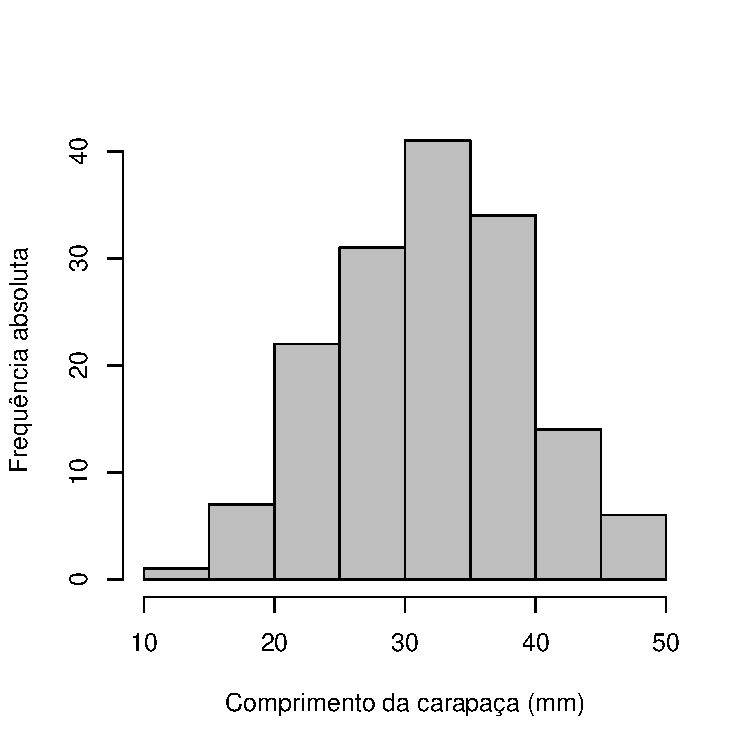
\includegraphics[width=.6\textwidth]{figure/unnamed-chunk-3} 

}


\end{knitrout}

\end{frame}

\begin{frame}[fragile=singleslide]{Testes de hipótese}{Teste-t
    para uma amostra}
Procedimentos gerais para um teste de hipótese
\begin{enumerate}
\item Definir a hipótese nula ($H_0$) e a alternativa ($H_1$)
\item Definir um nível de \textbf{significância} $\alpha$ (ex.: $\alpha
  = 0,05$), que irá determinar o nível de \textbf{confiança}
  $100(1-\alpha)\%$ do teste
\item Determinar a \textbf{região de rejeição} com base no nível de
  significância $\rightarrow$ $t_{crit}$
\item Calcula a \textbf{estatística de teste}, sob a hipótese nula
  \begin{equation*}
    t_{calc} = \frac{\bar{y} - \mu_0}{s/\sqrt{n}}
  \end{equation*}
\item Rejeitar a hipótese nula se a estatística de teste calculada
  estiver dentro da região de rejeição ($t_{calc} > t_{crit}$)
  \begin{itemize}
  \item Alternativamente, calcula-se o p-valor, que é a probabilidade de
    se obter um valor de $t$ igual ou maior do que $t_{calc}$
  \end{itemize}
\end{enumerate}
\end{frame}

\begin{frame}[fragile=singleslide]{Testes de hipótese}{Teste-t para uma
    amostra}
  \begin{itemize}
  \item Testar a hipótese de que a média ($\mu$) de CL é igual a 30 mm
    (com 95\% de confiança)
  \item As hipóteses são
    \begin{align*}
      H_0: \mu = 30 \\
      H_1: \mu \neq 30
    \end{align*}
  \end{itemize}
\end{frame}

\begin{frame}[fragile=singleslide]{Testes de hipótese}{Teste-t para uma
    amostra}
\begin{knitrout}\small
\definecolor{shadecolor}{rgb}{0.933, 0.914, 0.914}\color{fgcolor}\begin{kframe}
\begin{alltt}
> \hlfunctioncall{t.test}(dados$CL, mu = 30, alternative = \hlstring{"two.sided"},
         conf.level = 0.95)
\end{alltt}
\begin{verbatim}

	One Sample t-test

data:  dados$CL 
t = 3.4627, df = 155, p-value = 0.0006913
alternative hypothesis: true mean is not equal to 30 
95 percent confidence interval:
 30.861 33.147 
sample estimates:
mean of x 
   32.004 

\end{verbatim}
\end{kframe}
\end{knitrout}

\end{frame}

\begin{frame}[fragile=singleslide]{Testes de hipótese}{Teste-t para uma
    amostra}
\textbf{Detalhe:} O teste pode ser armazenado em um objeto para futuras
referências
\begin{knitrout}\small
\definecolor{shadecolor}{rgb}{0.933, 0.914, 0.914}\color{fgcolor}\begin{kframe}
\begin{alltt}
> teste <- \hlfunctioncall{t.test}(dados$CL, mu = 30, alternative = \hlstring{"two.sided"},
                  conf.level = 0.95)
> \hlfunctioncall{names}(teste)
\end{alltt}
\begin{verbatim}
[1] "statistic"   "parameter"   "p.value"     "conf.int"   
[5] "estimate"    "null.value"  "alternative" "method"     
[9] "data.name"  
\end{verbatim}
\begin{alltt}
> teste$statistic
\end{alltt}
\begin{verbatim}
     t 
3.4627 
\end{verbatim}
\begin{alltt}
> teste$p.value
\end{alltt}
\begin{verbatim}
[1] 0.00069135
\end{verbatim}
\end{kframe}
\end{knitrout}

\end{frame}

\begin{frame}[fragile=singleslide]{Testes de hipótese}{Teste-t para uma
    amostra}
  \begin{itemize}
  \item Testar a hipótese de que a média ($\mu$) de CL é menor do que 30
    mm (com 95\% de confiança)
  \item As hipóteses são
    \begin{align*}
      H_0: \mu \leq 30 \\
      H_1: \mu > 30
    \end{align*}
  \end{itemize}
\end{frame}

\begin{frame}[fragile=singleslide]{Testes de hipótese}{Teste-t para uma
    amostra}
\begin{knitrout}\small
\definecolor{shadecolor}{rgb}{0.933, 0.914, 0.914}\color{fgcolor}\begin{kframe}
\begin{alltt}
> \hlfunctioncall{t.test}(dados$CL, mu = 30, alternative = \hlstring{"greater"},
         conf.level = 0.95)
\end{alltt}
\begin{verbatim}

	One Sample t-test

data:  dados$CL 
t = 3.4627, df = 155, p-value = 0.0003457
alternative hypothesis: true mean is greater than 30 
95 percent confidence interval:
 31.046    Inf 
sample estimates:
mean of x 
   32.004 

\end{verbatim}
\end{kframe}
\end{knitrout}

\end{frame}

\begin{frame}[fragile=singleslide]{Testes de hipótese}{Teste-t para uma
    amostra}
  \begin{itemize}
  \item Testar a hipótese de que a média ($\mu$) de CL é maior do que 30
    mm (com 95\% de confiança)
  \item As hipóteses são
    \begin{align*}
      H_0: \mu \geq 30 \\
      H_1: \mu < 30
    \end{align*}
  \end{itemize}
\end{frame}

\begin{frame}[fragile=singleslide]{Testes de hipótese}{Teste-t para uma
    amostra}
\begin{knitrout}\small
\definecolor{shadecolor}{rgb}{0.933, 0.914, 0.914}\color{fgcolor}\begin{kframe}
\begin{alltt}
> \hlfunctioncall{t.test}(dados$CL, mu = 30, alternative = \hlstring{"less"},
         conf.level = 0.95)
\end{alltt}
\begin{verbatim}

	One Sample t-test

data:  dados$CL 
t = 3.4627, df = 155, p-value = 0.9997
alternative hypothesis: true mean is less than 30 
95 percent confidence interval:
   -Inf 32.961 
sample estimates:
mean of x 
   32.004 

\end{verbatim}
\end{kframe}
\end{knitrout}

\end{frame}

\begin{frame}[fragile=singleslide]{Testes de hipótese}{Teste-t para duas amostras}
\begin{knitrout}\small
\definecolor{shadecolor}{rgb}{0.933, 0.914, 0.914}\color{fgcolor}\begin{kframe}
\begin{alltt}
> \hlfunctioncall{require}(lattice) \hlcomment{# pacote para gráficos avançados}
> \hlfunctioncall{histogram}(~CL | especie, data = dados)
\end{alltt}
\end{kframe}

{\centering 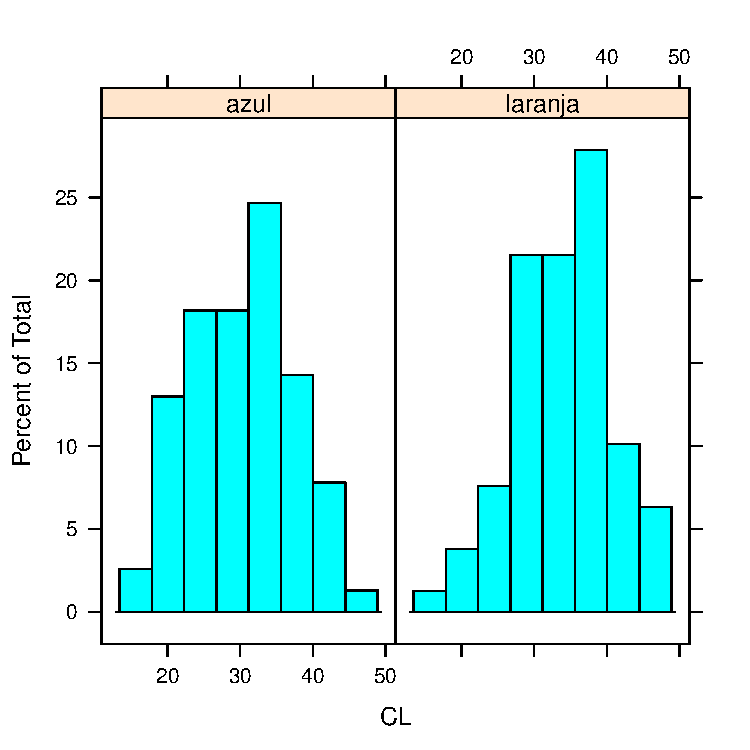
\includegraphics[width=.6\textwidth]{figure/unnamed-chunk-8} 

}


\end{knitrout}

\end{frame}

\begin{frame}[fragile=singleslide]{Testes de hipótese}{Teste-t para duas amostras}
\begin{knitrout}\small
\definecolor{shadecolor}{rgb}{0.933, 0.914, 0.914}\color{fgcolor}\begin{kframe}
\begin{alltt}
> \hlfunctioncall{with}(dados, \hlfunctioncall{tapply}(CL, especie, summary))
\end{alltt}
\begin{verbatim}
$azul
   Min. 1st Qu.  Median    Mean 3rd Qu.    Max. 
   14.7    24.6    30.1    29.9    34.5    47.1 

$laranja
   Min. 1st Qu.  Median    Mean 3rd Qu.    Max. 
   16.7    29.4    34.5    34.1    39.2    47.6 

\end{verbatim}
\end{kframe}
\end{knitrout}

Existem evidências de que uma espécie é maior do que a outra?
\end{frame}

\begin{frame}[fragile=singleslide]{Testes de hipótese}{Teste-t para duas amostras}
  \begin{itemize}
  \item Testar a hipótese de que a \textbf{diferença} entre a média de
    CL da espécie azul ($\mu_A$) e a média de CL da espécie laranja
    ($\mu_L$) é igual a 0 (zero) (com 95\% de confiança)
  \item As hipóteses são
    \begin{align*}
      H_0: \mu_A - \mu_L = 0 \quad \Rightarrow \quad \mu_A = \mu_L \\
      H_1: \mu_A - \mu_L \neq 0 \quad \Rightarrow \quad \mu_A \neq \mu_L
    \end{align*}
  \end{itemize}
\end{frame}

\begin{frame}[fragile=singleslide]{Testes de hipótese}{Teste-t para duas amostras}
\begin{knitrout}\small
\definecolor{shadecolor}{rgb}{0.933, 0.914, 0.914}\color{fgcolor}\begin{kframe}
\begin{alltt}
> \hlfunctioncall{t.test}(CL ~ especie, data = dados, mu = 0,
         alternative = \hlstring{"two.sided"}, conf.level = 0.95)
\end{alltt}
\begin{verbatim}

	Welch Two Sample t-test

data:  CL by especie 
t = -3.7935, df = 152.73, p-value = 0.0002135
alternative hypothesis: true difference in means is not equal to 0 
95 percent confidence interval:
 -6.4116 -2.0204 
sample estimates:
   mean in group azul mean in group laranja 
               29.869                34.085 

\end{verbatim}
\end{kframe}
\end{knitrout}

\end{frame}

\begin{frame}[fragile=singleslide]{Testes de hipótese}{Teste-t para duas amostras}
  \begin{itemize}
  \item Testar a hipótese de que a \textbf{diferença} entre a média de
    CL da espécie azul ($\mu_A$) e a média de CL da espécie laranja
    ($\mu_L$) é \textbf{menor} do que 0 (zero) (com 95\% de confiança)
  \item Em outras palavras: ``O CL médio é menor para a espécie azul?''
  \item As hipóteses são
    \begin{align*}
      H_0: \mu_A - \mu_L \leq 0 \quad \Rightarrow \quad \mu_A \leq \mu_L \\
      H_1: \mu_A - \mu_L > 0 \quad \Rightarrow \quad \mu_A > \mu_L
    \end{align*}
  \end{itemize}
\end{frame}

\begin{frame}[fragile=singleslide]{Testes de hipótese}{Teste-t para duas amostras}
\begin{knitrout}\small
\definecolor{shadecolor}{rgb}{0.933, 0.914, 0.914}\color{fgcolor}\begin{kframe}
\begin{alltt}
> \hlfunctioncall{t.test}(CL ~ especie, data = dados, mu = 0,
         alternative = \hlstring{"greater"}, conf.level = 0.95)
\end{alltt}
\begin{verbatim}

	Welch Two Sample t-test

data:  CL by especie 
t = -3.7935, df = 152.73, p-value = 0.9999
alternative hypothesis: true difference in means is greater than 0 
95 percent confidence interval:
 -6.0552     Inf 
sample estimates:
   mean in group azul mean in group laranja 
               29.869                34.085 

\end{verbatim}
\end{kframe}
\end{knitrout}

Como você faria para calcular a diferença observada das médias de CL
entre as duas espécies?
\end{frame}

\begin{frame}[fragile=singleslide]{Exercícios}
Com base no objeto \texttt{dados}:
  \begin{enumerate}
  \item Faça um histograma de CW
  \item Com base no histograma, construa uma hipótese para a média de CW
    \begin{enumerate}
    \item Teste a igualdade dessa hipótese
    \item Teste uma desigualdade dessa hipótese
    \end{enumerate}
    Em ambos os casos use um nível de confiança de 90\%, e escreva uma
    frase com a sua conclusão.
  \item Faça um histograma de CW para cada sexo
  \item Com base nesses histogramas, construa uma hipótese para a
    diferença média de CW entre os sexos
    \begin{enumerate}
    \item Teste a igualdade dessa hipótese
    \item Teste uma desigualdade dessa hipótese
    \end{enumerate}
    Em ambos os casos use um nível de confiança de 90\%, e escreva uma
    frase com a sua conclusão.
  \end{enumerate}
\end{frame}

\section{Correlação e regressão}

\begin{frame}[fragile=singleslide]{Correlação e regressão}
Vamos analisar a correlação que existe entre CL e CW
\begin{knitrout}\small
\definecolor{shadecolor}{rgb}{0.933, 0.914, 0.914}\color{fgcolor}\begin{kframe}
\begin{alltt}
> \hlfunctioncall{plot}(CW ~ CL, data = dados)
\end{alltt}
\end{kframe}

{\centering 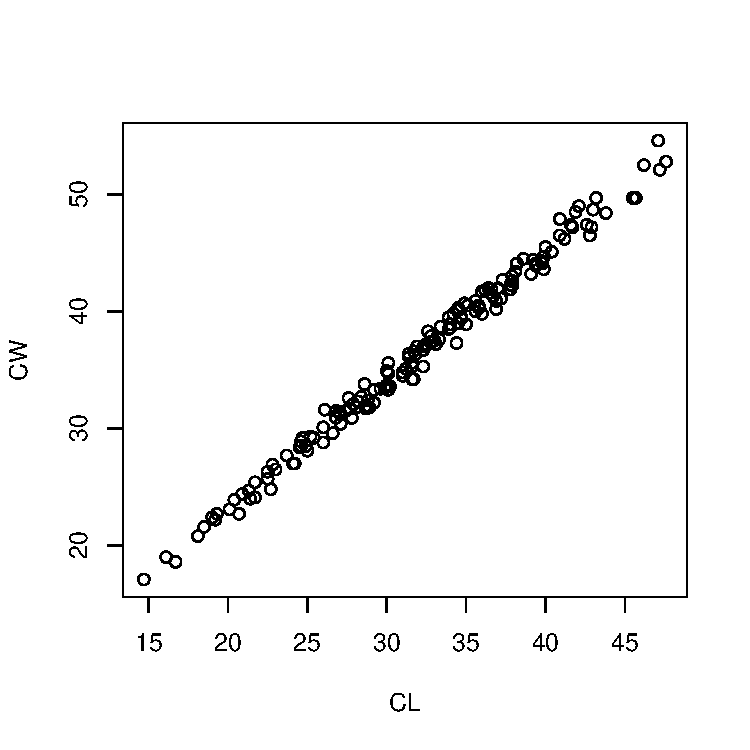
\includegraphics[width=.6\textwidth]{figure/unnamed-chunk-12} 

}


\end{knitrout}

\end{frame}

\begin{frame}[fragile=singleslide]{Correlação}
A correlação entre duas variáveis é simbolizada por $\rho$ (para a
população) e $r$ (para a amostra), e varia no intervalo $[-1,1]$
\begin{equation*}
  r = \frac{\sum (x_i - \bar{x})(y_i - \bar{y})}
  {\sqrt{\sum (x_i - \bar{x})^2 \sum (y_i - \bar{y})^2}}
\end{equation*}
\begin{knitrout}\small
\definecolor{shadecolor}{rgb}{0.933, 0.914, 0.914}\color{fgcolor}

{\centering 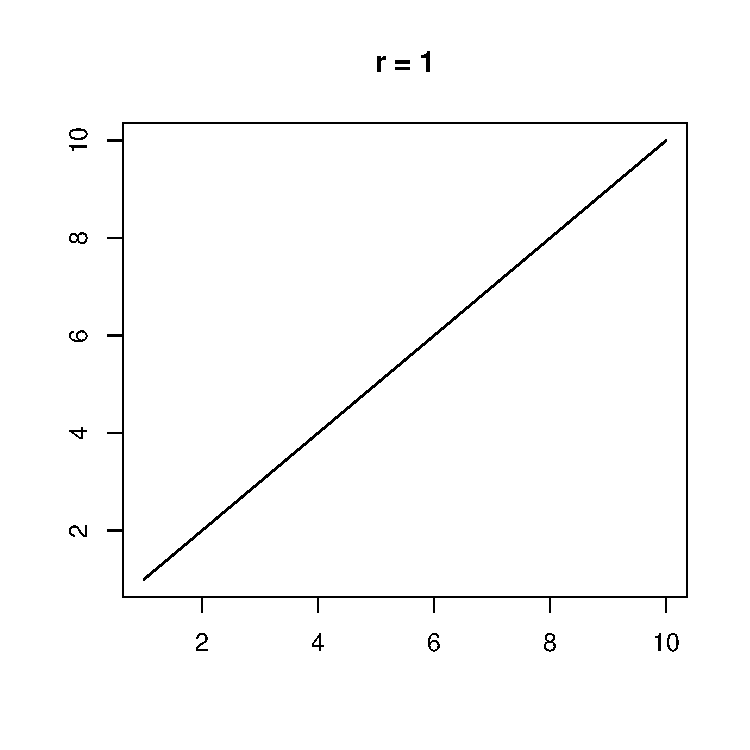
\includegraphics[width=.33\textwidth]{figure/unnamed-chunk-131} 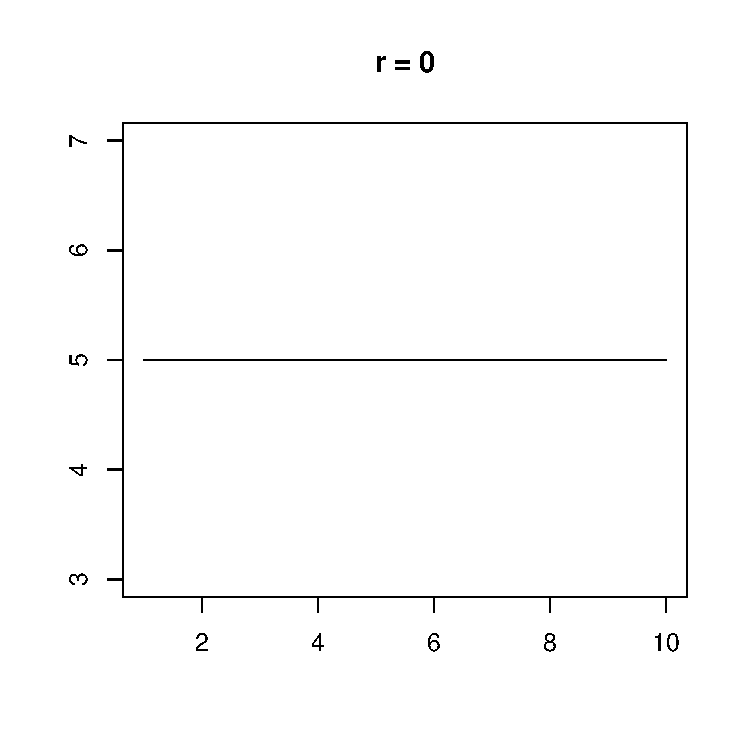
\includegraphics[width=.33\textwidth]{figure/unnamed-chunk-132} 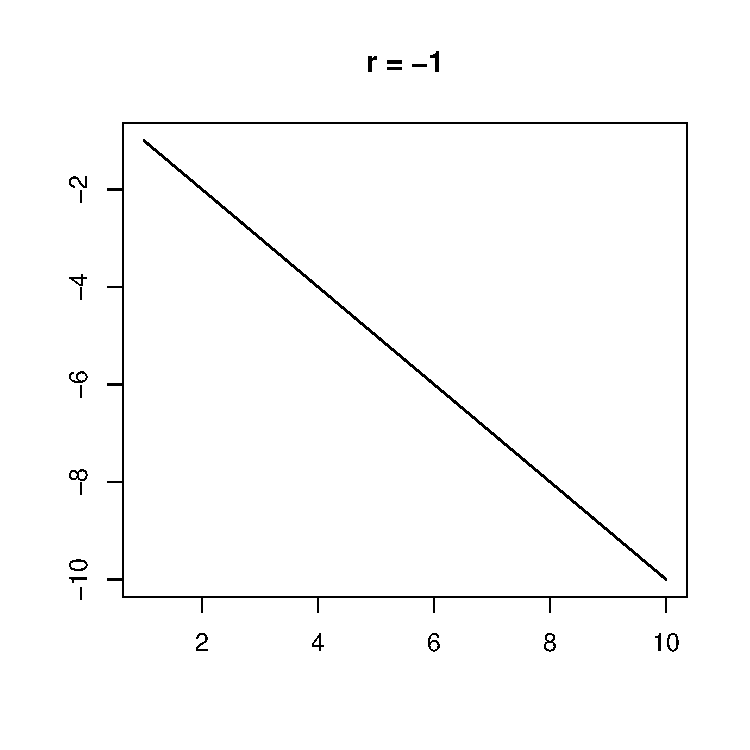
\includegraphics[width=.33\textwidth]{figure/unnamed-chunk-133} 

}


\end{knitrout}

Portanto, um \textbf{teste de correlação} tem as seguintes hipóteses
\begin{align*}
  H_0: \rho = 0 \\
  H_1: \rho \neq 0
\end{align*}
\end{frame}

\begin{frame}[fragile=singleslide]{Correlação}
Teste de correlação entre CL e CW
\begin{knitrout}\small
\definecolor{shadecolor}{rgb}{0.933, 0.914, 0.914}\color{fgcolor}\begin{kframe}
\begin{alltt}
> \hlfunctioncall{cor}(dados$CL, dados$CW)
\end{alltt}
\begin{verbatim}
[1] 0.9952
\end{verbatim}
\begin{alltt}
> \hlfunctioncall{cor.test}(dados$CL, dados$CW)
\end{alltt}
\begin{verbatim}

	Pearson's product-moment correlation

data:  dados$CL and dados$CW 
t = 126.17, df = 154, p-value < 2.2e-16
alternative hypothesis: true correlation is not equal to 0 
95 percent confidence interval:
 0.99341 0.99650 
sample estimates:
   cor 
0.9952 

\end{verbatim}
\end{kframe}
\end{knitrout}

\end{frame}

\begin{frame}[fragile=singleslide]{Regressão}
O modelo linear é definido por:
\begin{equation*}
  y_i = \beta_0 + \beta_1 x_{i} + \epsilon_i
\end{equation*}
onde
\begin{itemize}
\item $y$ é a variável resposta
\item $x$ é a variável explicativa
\item $\beta_0$ é o intercepto da reta (valor de $y$ quando $x = 0$)
\item $\beta_1$ é a inclinação da reta (\textbf{efeito} de $x$ sobre $y$)
\item $i = 1, 2, \ldots, n$ observações
\item $\epsilon \sim N(0, \sigma^2)$
\end{itemize}
\end{frame}

\begin{frame}[fragile=singleslide]{Regressão}
Os parâmetros $\beta_0$ e $\beta_1$ são estimados pelo \textbf{método dos
mínimos quadrados}. Os resíduos são
\begin{equation*}
  \epsilon_i = y_i - (\beta_0 - \beta_1 x_i)
\end{equation*}
Portanto, a \textbf{soma dos quadrados dos resíduos} (SQR) é
\begin{equation*}
  SQR = \sum_{i=1}^{n} (y_i - (\beta_0 - \beta_1 x_i))^2
\end{equation*}
Através das derivadas da SQR em relação à $\beta_0$ e $\beta_1$ chega-se
aos resultados
\begin{align*}
  \hat{\beta_1} &= \frac{\sum (y_i - \bar{y}) (x_i - \bar{x})}
  {\sum (x_i - \bar{x})^2} \\
  \hat{\beta_0} &= \bar{y} - \hat{\beta_1} \bar{x}
\end{align*}
\end{frame}

\begin{frame}[fragile=singleslide]{Regressão}
Ajustando um modelo linear no \R
\begin{knitrout}\small
\definecolor{shadecolor}{rgb}{0.933, 0.914, 0.914}\color{fgcolor}\begin{kframe}
\begin{alltt}
> mod <- \hlfunctioncall{lm}(CW ~ CL, data = dados)
> mod
\end{alltt}
\begin{verbatim}

Call:
lm(formula = CW ~ CL, data = dados)

Coefficients:
(Intercept)           CL  
       1.19         1.10  

\end{verbatim}
\end{kframe}
\end{knitrout}

\end{frame}

\begin{frame}[fragile=singleslide]{Regressão}{Sumário}
\begin{knitrout}\footnotesize
\definecolor{shadecolor}{rgb}{0.933, 0.914, 0.914}\color{fgcolor}\begin{kframe}
\begin{alltt}
> \hlfunctioncall{summary}(mod)
\end{alltt}
\begin{verbatim}

Call:
lm(formula = CW ~ CL, data = dados)

Residuals:
   Min     1Q Median     3Q    Max 
-1.776 -0.570  0.110  0.463  1.827 

Coefficients:
            Estimate Std. Error t value Pr(>|t|)    
(Intercept)   1.1869     0.2853    4.16  5.3e-05 ***
CL            1.0975     0.0087  126.17  < 2e-16 ***
---
Signif. codes:  0 '***' 0.001 '**' 0.01 '*' 0.05 '.' 0.1 ' ' 1 

Residual standard error: 0.783 on 154 degrees of freedom
Multiple R-squared: 0.99,	Adjusted R-squared: 0.99 
F-statistic: 1.59e+04 on 1 and 154 DF,  p-value: <2e-16 

\end{verbatim}
\end{kframe}
\end{knitrout}

\end{frame}

\begin{frame}[fragile=singleslide]{Regressão}{Ajuste gráfico}
\begin{knitrout}\small
\definecolor{shadecolor}{rgb}{0.933, 0.914, 0.914}\color{fgcolor}\begin{kframe}
\begin{alltt}
> \hlfunctioncall{plot}(CW ~ CL, data = dados)
> \hlfunctioncall{abline}(mod)
> \hlfunctioncall{plot}(CW ~ CL, data = dados, xlim = \hlfunctioncall{c}(0,50), ylim = \hlfunctioncall{c}(0,55))
> \hlfunctioncall{abline}(mod)
\end{alltt}
\end{kframe}

{\centering 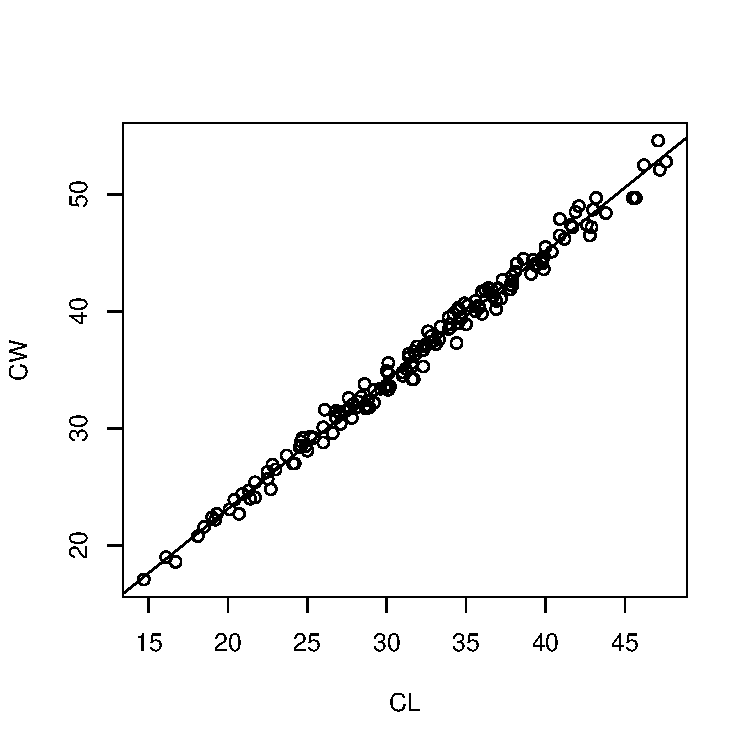
\includegraphics[width=.49\textwidth]{figure/unnamed-chunk-171} 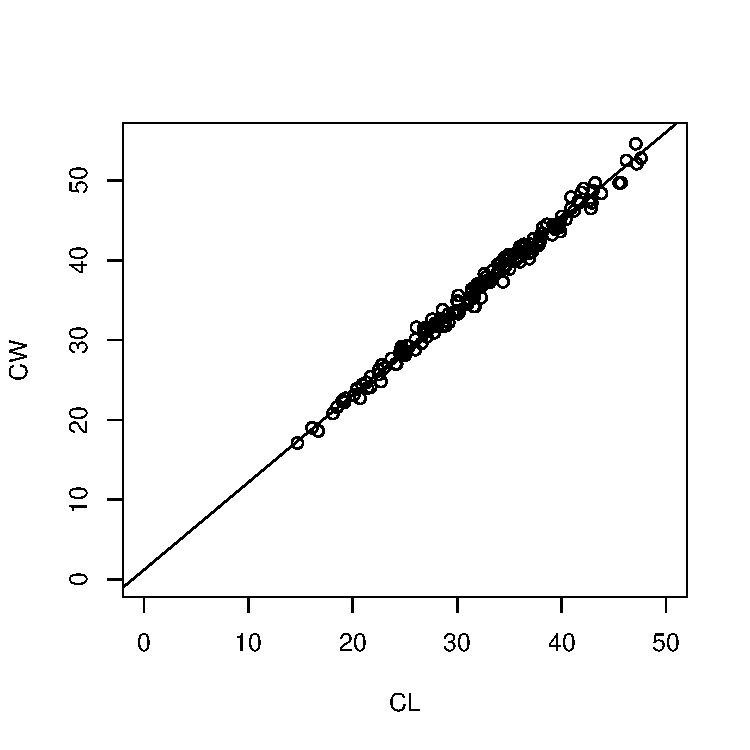
\includegraphics[width=.49\textwidth]{figure/unnamed-chunk-172} 

}


\end{knitrout}

\end{frame}

\begin{frame}[fragile=singleslide]{Regressão}{Análise dos resíduos}
\begin{knitrout}\small
\definecolor{shadecolor}{rgb}{0.933, 0.914, 0.914}\color{fgcolor}\begin{kframe}
\begin{alltt}
> \hlfunctioncall{par}(mfrow = \hlfunctioncall{c}(2,2))
> \hlfunctioncall{plot}(mod)
> \hlfunctioncall{par}(mfrow = \hlfunctioncall{c}(1,1))
\end{alltt}
\end{kframe}

{\centering 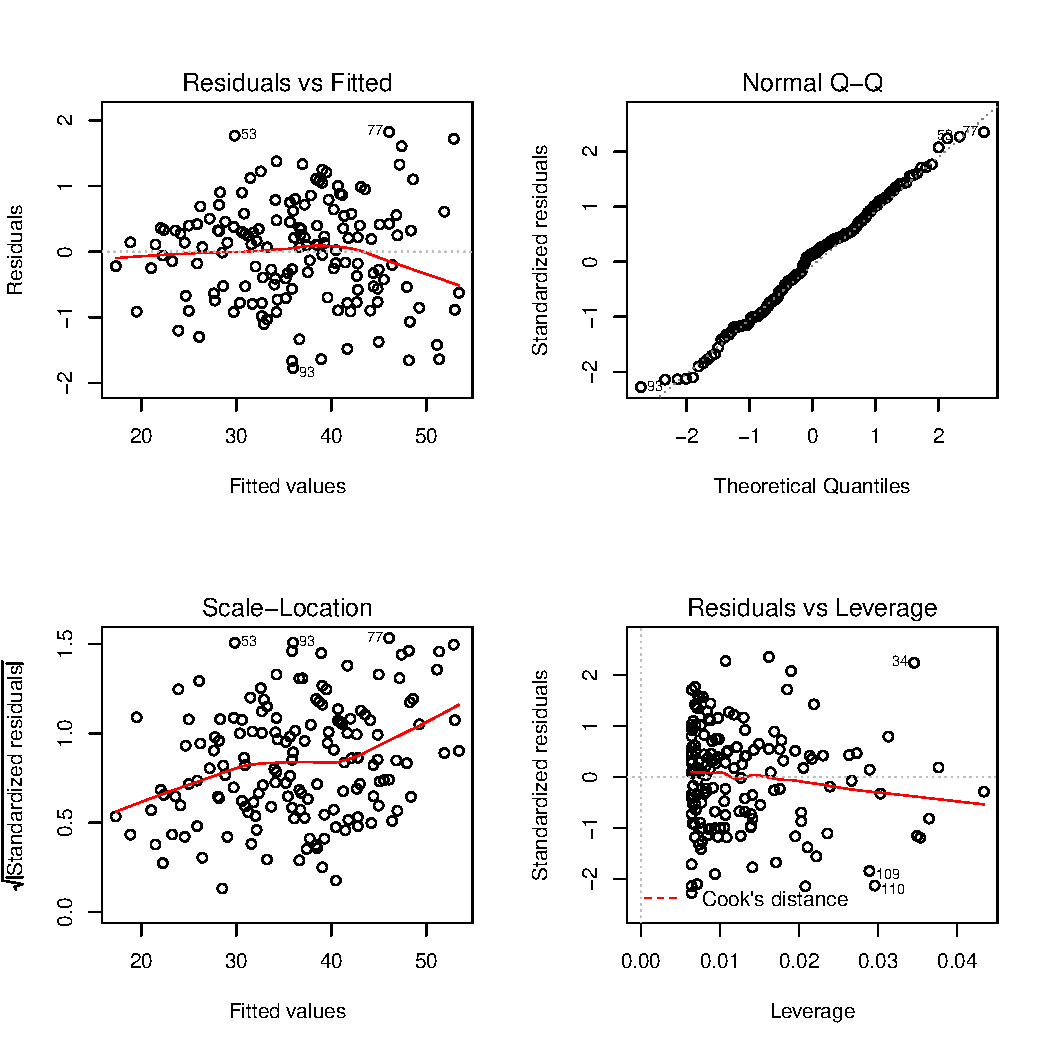
\includegraphics[width=.6\textwidth]{figure/unnamed-chunk-18} 

}


\end{knitrout}

\end{frame}

\begin{frame}[fragile=singleslide]{Regressão}
Acessando os componentes do objeto \texttt{mod}:
\begin{knitrout}\small
\definecolor{shadecolor}{rgb}{0.933, 0.914, 0.914}\color{fgcolor}\begin{kframe}
\begin{alltt}
> \hlfunctioncall{names}(mod)
\end{alltt}
\begin{verbatim}
 [1] "coefficients"  "residuals"     "effects"      
 [4] "rank"          "fitted.values" "assign"       
 [7] "qr"            "df.residual"   "xlevels"      
[10] "call"          "terms"         "model"        
\end{verbatim}
\begin{alltt}
> \hlfunctioncall{names}(\hlfunctioncall{summary}(mod))
\end{alltt}
\begin{verbatim}
 [1] "call"          "terms"         "residuals"    
 [4] "coefficients"  "aliased"       "sigma"        
 [7] "df"            "r.squared"     "adj.r.squared"
[10] "fstatistic"    "cov.unscaled" 
\end{verbatim}
\end{kframe}
\end{knitrout}

\end{frame}

\begin{frame}[fragile=singleslide]{Exercícios}
Com as colunas BD e CL do objeto \texttt{dados}
\begin{enumerate}
\item Faça um gráfico da relação entre estas variáveis
\item Faça um teste de correlação
\item Ajuste um modelo linear
  \begin{enumerate}
  \item Veja o sumário
  \item Ajuste a linha do modelo no gráfico
  \item Verifique os resíduos
  \end{enumerate}
\end{enumerate}
Qual sua conclusão?
\small
\begin{itemize}
\item Existe correlação significativa? De que tipo (positiva, negativa)?
\item O modelo linear descreve bem a relação entre estas duas variáveis
  (verifique com o valor de \verb+Pr(>|t|)+ e do $R^2$)
\item O modelos foi bem ajustado aos dados (observe os resíduos)
\end{itemize}
\end{frame}


\section[ANOVA]{Análise de Variância}

%\begin{frame}[fragile=singleslide]{Análise de Variância}{Base de dados}
%<<>>=
%## dados <- read.table("crabs.csv", header = T, sep = ";",
%##                     dec = ",")
%## str(dados)
%@
%\end{frame}

\begin{frame}[fragile=singleslide]{Análise de Variância}
Definição: $y_{ij}$ representa a observação $j$ do grupo $i$;
$\bar{y}_{i}$ é a média do grupo $i$; $\bar{y}$ é a média geral de todas
as observações. As observações podem ser decompostas em
\begin{equation*}
  y_{ij} = \quad \bar{y} \quad + \quad (\bar{y}_{i} - \bar{y}) \quad + \quad
  (y_{ij} - \bar{y}_{i})
\end{equation*}
que corresponde ao modelo
\begin{equation*}
  y_{ij} = \quad \theta \quad + \quad \mu_i \quad + \quad \epsilon_{ij},
  \qquad \epsilon_{ij} \sim N(0, \sigma^2)
\end{equation*}
A hipótese a ser testada de que todos os grupos são iguais (\textit{i.e}
médias iguais) implica que todos os $\mu_{i}$ são iguais:
\begin{align*}
  &H_0: \mu_1 = \mu_2 = \cdots = \mu_n \\
  &H_1: \textsf{pelo menos um}\ \mu_i\ \textsf{é diferente dos demais}
\end{align*}
\end{frame}

\begin{frame}[fragile=singleslide]{Análise de Variância}
Voltando ao exemplo da diferença de CL entre as duas espécies:\\
$\bar{y}_A = 29.9$ e
$\bar{y}_L = 34.1$
\begin{knitrout}\small
\definecolor{shadecolor}{rgb}{0.933, 0.914, 0.914}\color{fgcolor}\begin{kframe}
\begin{alltt}
> \hlfunctioncall{with}(dados, \hlfunctioncall{tapply}(CL, especie, summary))
\end{alltt}
\begin{verbatim}
$azul
   Min. 1st Qu.  Median    Mean 3rd Qu.    Max. 
   14.7    24.6    30.1    29.9    34.5    47.1 

$laranja
   Min. 1st Qu.  Median    Mean 3rd Qu.    Max. 
   16.7    29.4    34.5    34.1    39.2    47.6 

\end{verbatim}
\end{kframe}
\end{knitrout}

Média geral $\bar{y} = 32$
\begin{knitrout}\small
\definecolor{shadecolor}{rgb}{0.933, 0.914, 0.914}\color{fgcolor}\begin{kframe}
\begin{alltt}
> \hlfunctioncall{mean}(dados$CL)
\end{alltt}
\begin{verbatim}
[1] 32.004
\end{verbatim}
\end{kframe}
\end{knitrout}

\end{frame}

\begin{frame}[fragile=singleslide]{Análise de Variância}
\begin{knitrout}\small
\definecolor{shadecolor}{rgb}{0.933, 0.914, 0.914}\color{fgcolor}\begin{kframe}
\begin{alltt}
> \hlfunctioncall{boxplot}(CL ~ especie, data = dados)
> \hlfunctioncall{abline}(h = \hlfunctioncall{mean}(dados$CL), lty = 2, col = \hlstring{"red"}, lwd = 2)
\end{alltt}
\end{kframe}

{\centering 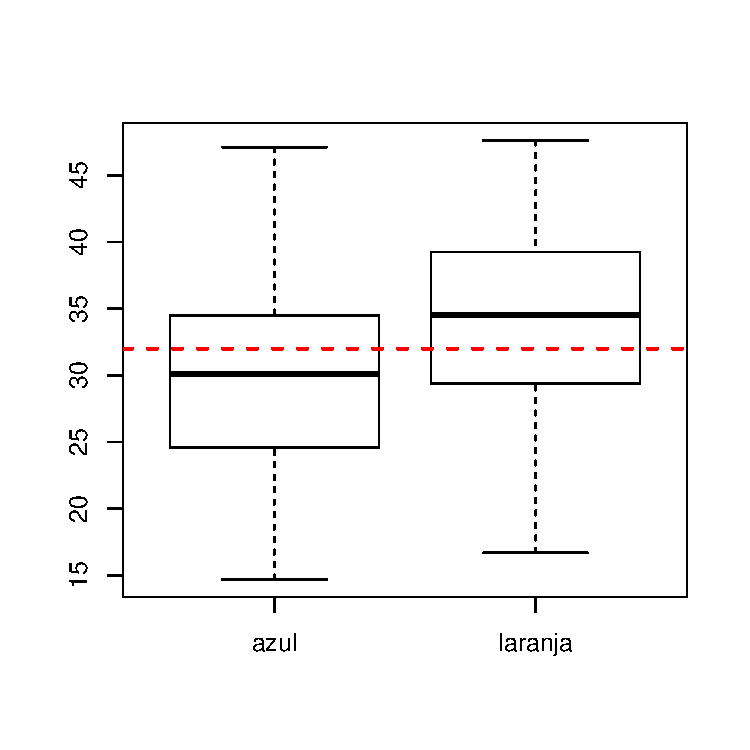
\includegraphics[width=.6\textwidth]{figure/unnamed-chunk-22} 

}


\end{knitrout}

\end{frame}

\begin{frame}[fragile=singleslide]{Análise de Variância}
Geometricamente
\begin{knitrout}\small
\definecolor{shadecolor}{rgb}{0.933, 0.914, 0.914}\color{fgcolor}

{\centering 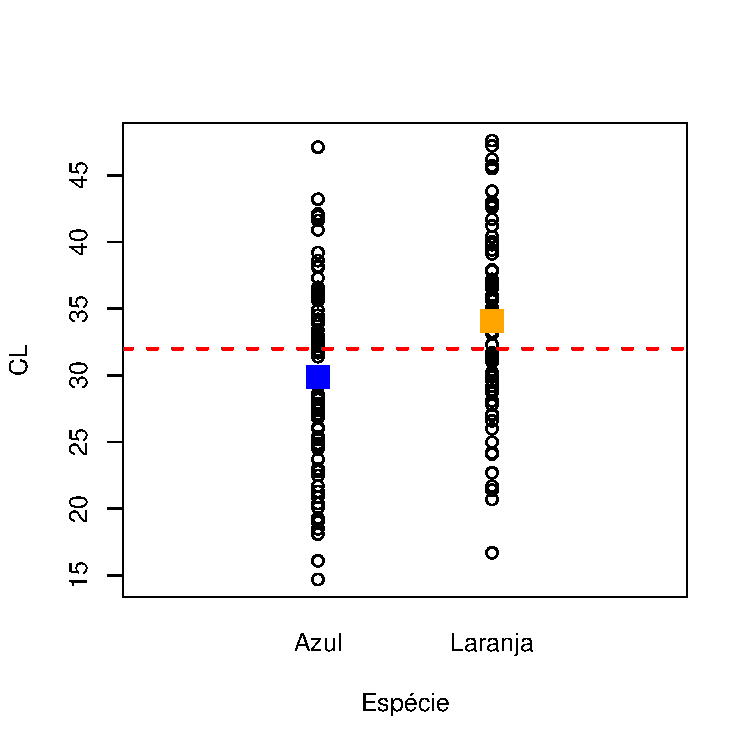
\includegraphics[width=.7\textwidth]{figure/unnamed-chunk-23} 

}


\end{knitrout}

\end{frame}

\begin{frame}[fragile=singleslide]{Análise de Variância}
Podemos ajustar um modelo linear entre CL e espécie
\begin{knitrout}\footnotesize
\definecolor{shadecolor}{rgb}{0.933, 0.914, 0.914}\color{fgcolor}\begin{kframe}
\begin{alltt}
> mod <- \hlfunctioncall{lm}(CL ~ especie, data = dados)
> \hlfunctioncall{summary}(mod)
\end{alltt}
\begin{verbatim}

Call:
lm(formula = CL ~ especie, data = dados)

Residuals:
    Min      1Q  Median      3Q     Max 
-17.385  -5.019   0.273   5.019  17.231 

Coefficients:
               Estimate Std. Error t value Pr(>|t|)    
(Intercept)       29.87       0.79    37.8  < 2e-16 ***
especielaranja     4.22       1.11     3.8  0.00021 ***
---
Signif. codes:  0 '***' 0.001 '**' 0.01 '*' 0.05 '.' 0.1 ' ' 1 

Residual standard error: 6.93 on 154 degrees of freedom
Multiple R-squared: 0.0856,	Adjusted R-squared: 0.0797 
F-statistic: 14.4 on 1 and 154 DF,  p-value: 0.00021 

\end{verbatim}
\end{kframe}
\end{knitrout}

\end{frame}

\begin{frame}[fragile=singleslide]{Análise de Variância}
Ajustando o modelo
\begin{knitrout}\small
\definecolor{shadecolor}{rgb}{0.933, 0.914, 0.914}\color{fgcolor}

{\centering 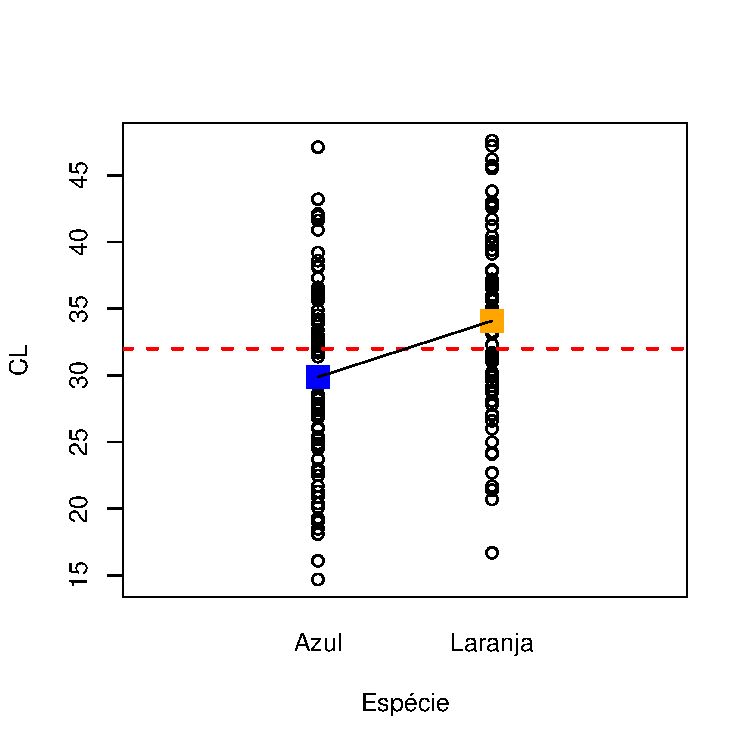
\includegraphics[width=.7\textwidth]{figure/unnamed-chunk-25} 

}


\end{knitrout}

\end{frame}

\begin{frame}[fragile=singleslide]{Análise de Variância}
Você lembra do teste-t feito anteriormente?
\begin{knitrout}\footnotesize
\definecolor{shadecolor}{rgb}{0.933, 0.914, 0.914}\color{fgcolor}\begin{kframe}
\begin{alltt}
> teste <- \hlfunctioncall{t.test}(CL ~ especie, data = dados, mu = 0,
                  alternative = \hlstring{"two.sided"}, conf.level = 0.95)
> teste
\end{alltt}
\begin{verbatim}

	Welch Two Sample t-test

data:  CL by especie 
t = -3.7935, df = 152.73, p-value = 0.0002135
alternative hypothesis: true difference in means is not equal to 0 
95 percent confidence interval:
 -6.4116 -2.0204 
sample estimates:
   mean in group azul mean in group laranja 
               29.869                34.085 

\end{verbatim}
\end{kframe}
\end{knitrout}

\end{frame}

\begin{frame}[fragile=singleslide]{Análise de Variância}
Notou a relação?
\begin{knitrout}\footnotesize
\definecolor{shadecolor}{rgb}{0.933, 0.914, 0.914}\color{fgcolor}\begin{kframe}
\begin{alltt}
> \hlfunctioncall{summary}(mod)$coefficients
\end{alltt}
\begin{verbatim}
               Estimate Std. Error t value   Pr(>|t|)
(Intercept)      29.869     0.7902 37.7990 8.1924e-80
especielaranja    4.216     1.1104  3.7968 2.1042e-04
\end{verbatim}
\begin{alltt}
> teste$p.value
\end{alltt}
\begin{verbatim}
[1] 2.1352e-04
\end{verbatim}
\begin{alltt}
> teste$estimate
\end{alltt}
\begin{verbatim}
   mean in group azul mean in group laranja 
               29.869                34.085 
\end{verbatim}
\begin{alltt}
> \hlfunctioncall{diff}(teste$estimate)
\end{alltt}
\begin{verbatim}
mean in group laranja 
                4.216 
\end{verbatim}
\end{kframe}
\end{knitrout}

\end{frame}

\begin{frame}[fragile=singleslide]{Análise de Variância}
A ANOVA vai testar apenas a hipótese inicial
\begin{align*}
  &H_0: \mu_A = \mu_L \\
  &H_1: \mu_A \neq \mu_L
\end{align*}
\begin{knitrout}\small
\definecolor{shadecolor}{rgb}{0.933, 0.914, 0.914}\color{fgcolor}\begin{kframe}
\begin{alltt}
> \hlfunctioncall{anova}(mod)
\end{alltt}
\begin{verbatim}
Analysis of Variance Table

Response: CL
           Df Sum Sq Mean Sq F value  Pr(>F)    
especie     1    693     693    14.4 0.00021 ***
Residuals 154   7404      48                    
---
Signif. codes:  0 '***' 0.001 '**' 0.01 '*' 0.05 '.' 0.1 ' ' 1 
\end{verbatim}
\end{kframe}
\end{knitrout}

Aqui a única conclusão é de que os $\mu_i$ não são iguais (mas você
não sabe quanto e nem quais!)
\end{frame}

\begin{frame}[fragile=singleslide]{Análise de Variância}
Se olharmos apenas o resultado da ANOVA, podemos prosseguir com a
análise fazendo um teste \textit{a posteriori} para verificarmos quais
são os grupos que diferem entre si. Um deles é o teste de Tukey
\begin{knitrout}\small
\definecolor{shadecolor}{rgb}{0.933, 0.914, 0.914}\color{fgcolor}\begin{kframe}
\begin{alltt}
> mod.anova <- \hlfunctioncall{aov}(CL ~ especie, data = dados)
> \hlfunctioncall{TukeyHSD}(mod.anova)
\end{alltt}
\begin{verbatim}
  Tukey multiple comparisons of means
    95% family-wise confidence level

Fit: aov(formula = CL ~ especie, data = dados)

$especie
              diff    lwr    upr   p adj
laranja-azul 4.216 2.0224 6.4096 0.00021

\end{verbatim}
\end{kframe}
\end{knitrout}

\end{frame}

\begin{frame}[fragile=singleslide]{Análise de Variância}
Porque então fazer uma ANOVA???
\begin{itemize}
\item Quando formos comparar a média de mais de 2 grupos
\item Não é possível fazer um teste-t para mais de 2 grupos
\item Por exemplo, com 3 grupos (A, B, C) teríamos que fazer 3
  comparações (A:B, A:C, B:C)
  \begin{itemize}
  \item Com um nível de confiança de 95\% ($\alpha = 0.05$)
    para cada teste, os 3 testes teriam um nível de confiança
    $(1-\alpha)^3$
  \item Portanto $(1-0.05)^3 = (0.95)^3 = 0.85$
  \item Isso implica que quanto mais comparações forem feitas, menor
    será seu nível de confiança no resultado dos testes.
  \end{itemize}
\end{itemize}
\end{frame}

\section[MLGs]{Modelos Lineares Generalizados}

\begin{frame}[fragile=singleslide]{Modelos Lineares Generalizados}
Nelder e Wedderburn (1972) mostraram que uma série de técnicas
estatísticas podem ser formuladas de forma unificada, como uma classe de
modelos de regressão. A essa teoria, uma extensão dos modelos clássicos
de regressão, deram o nome de \textbf{Modelos Lineares
  Generalizados}.
\begin{center}
  Teste-t $\subset$ ANOVA $\subset$ ANCOVA* $\subset$ ML $\subset$
  ML-MULT* $\subset$ MLG
\end{center}
  \begin{itemize}
  \item Teste-t: compara uma ou duas médias
  \item ANOVA: compara 2 ou mais médias (fator)
  \item ANCOVA: compara 2 ou mais médias (fator) + variáveis numéricas
  \item ML: regressão de $y$ (numérico) em função de um único $x$
    (numérico ou fator)
  \item ML-MULT: regressão de $y$ (numérico) em função de mais de um $x$
    (numéricos ou fatores)
  \item MLG: Similar ao ML-MULT, mas extende o modelo para que $y$ possa
    ser um fator ou ter uma distribuição diferente da normal.
  \end{itemize}
\end{frame}

\begin{frame}[fragile=singleslide]{Modelos Lineares Generalizados}
Os MLGs são formados por três componentes:
\begin{enumerate}
\item \textbf{Componente aleatório}: a variável resposta do modelo, com
  distribuição pertencente à família de distribuições exponencial.
\item \textbf{Componente sistemático}: as variáveis explicativas, que
  entram na forma de uma estrutura linear.
\item \textbf{Função de ligação}: função que liga os componentes
  aleatório e sistemático.
\end{enumerate}
\end{frame}

\begin{frame}[fragile=singleslide]{Modelos Lineares Generalizados}
De maneira geral, os MLGs descrevem a relação entre a variável resposta
$y_i$ ($i = 1, \ldots, n$) através de preditores $x_i$. A média de $y_i$
condicionada aos preditores $x_i$ é
\begin{equation*}
  E(y_i|x_i) = \mu_i
\end{equation*}
e existe uma transformação de $\mu_i$ de forma que
\begin{equation*}
  g(\mu_i) = x_{i}^{T}\beta
\end{equation*}
onde $g(\cdot)$ é uma função de ligação conhecida, e $\beta$ é o vetor
de parâmetros a ser estimado.
\end{frame}

\begin{frame}[fragile=singleslide]{Modelos Lineares Generalizados}
Distribuições da família exponencial e funções de ligação (P = link
padrão)
\begin{center}
\begin{table}[h!]
\renewcommand{\baselinestretch}{1}
\small\footnotesize\scriptsize
\begin{tabular}{lcccccc}
\hline
Link & \texttt{binomial} & \texttt{poisson} & \texttt{negative} &
\texttt{Gamma} & \texttt{gaussian} & \texttt{inverse}\\
    &       &    & \texttt{binomial} &  &  & \texttt{gaussian} \\
\hline
\texttt{logit} & P & & & & & \\
\texttt{probit} & $\bullet$ & & & & &  \\
\texttt{cloglog} & $\bullet$ & & & & &  \\
\texttt{identity} &  & $\bullet$ & $\bullet$ & $\bullet$ & P &  \\
\texttt{inverse} &  & & & P & &  \\
\texttt{log} &  & P & P & $\bullet$ & &  \\
\verb|1/mu^2| & & & & & & P  \\
\texttt{sqrt} & & $\bullet$ & $\bullet$ & & &  \\
\hline
\end{tabular}
\end{table}
\end{center}
\end{frame}

\begin{frame}[fragile=singleslide]{Modelos Lineares Generalizados}
Para ajustar um MLG usamos a função \texttt{glm()}
\begin{knitrout}\footnotesize
\definecolor{shadecolor}{rgb}{0.933, 0.914, 0.914}\color{fgcolor}\begin{kframe}
\begin{alltt}
> mod.glm <- \hlfunctioncall{glm}(CL ~ especie, data = dados,
                 family = \hlfunctioncall{gaussian}(link = \hlstring{"identity"}))
> \hlfunctioncall{summary}(mod.glm)
\end{alltt}
\begin{verbatim}

Call:
glm(formula = CL ~ especie, family = gaussian(link = "identity"), 
    data = dados)

Deviance Residuals: 
    Min       1Q   Median       3Q      Max  
-17.385   -5.019    0.273    5.019   17.231  

Coefficients:
               Estimate Std. Error t value Pr(>|t|)    
(Intercept)       29.87       0.79    37.8  < 2e-16 ***
especielaranja     4.22       1.11     3.8  0.00021 ***
---
Signif. codes:  0 '***' 0.001 '**' 0.01 '*' 0.05 '.' 0.1 ' ' 1 

(Dispersion parameter for gaussian family taken to be 48.08)

    Null deviance: 8097.4  on 155  degrees of freedom
Residual deviance: 7404.3  on 154  degrees of freedom
AIC: 1051

Number of Fisher Scoring iterations: 2

\end{verbatim}
\end{kframe}
\end{knitrout}

\end{frame}

\begin{frame}[fragile=singleslide]{Modelos Lineares Generalizados}
Quando existe mais de uma variável resposta ($y$)? \textbf{Métodos
  multivariados}!
\end{frame}

\begin{frame}[fragile=singleslide]{Exercícios}
Com o objeto \texttt{dados}
\begin{enumerate}
\item Faça um boxplot de CW por sexo
\item Faça um teste-t para testar se existe diferença entre as médias de
  CW para machos e fêmeas
\item Ajuste um modelo linear para testar essa mesma hipótese
\item Faça uma ANOVA e o teste de Tukey
\end{enumerate}
Qual sua conclusão?
\end{frame}



% \section[ANOVA]{Análise de Variância}

% \begin{frame}[fragile=singleslide]{Análise de Variância}
% Definição: $y_{ij}$ representa a observação $j$ do grupo $i$;
% $\bar{y}_{i}$ é a média do grupo $i$; $\bar{y}$ é a média geral de todas
% as observações. As observações podem ser decompostas em
% \begin{equation*}
%   y_{ij} = \quad \bar{y} \quad + \quad (\bar{y}_{i} - \bar{y}) \quad + \quad
%   (y_{ij} - \bar{y}_{i})
% \end{equation*}
% que corresponde ao modelo
% \begin{equation*}
%   y_{ij} = \quad \mu \quad + \quad \alpha_i \quad + \quad \epsilon_{ij},
%   \qquad \epsilon_{ij} \sim N(0, \sigma^2)
% \end{equation*}
% A hipótese a ser testada de que todos os grupos são iguais (\textit{i.e}
% médias iguais) implica que todos os $\alpha_{i}$ são zero:
% \begin{align*}
%   &H_0: \alpha_1 = \alpha_2 = \cdots = \alpha_n = 0 \\
%   &H_1: \textsf{pelo menos um}\ \alpha_i\ \textsf{é diferente dos demais}
% \end{align*}
% \end{frame}

% \begin{frame}[fragile=singleslide]{Análise de Variância}
% Voltando ao exemplo da diferença de CL entre as duas espécies
% <<>>=
% with(dados, tapply(CL, especie, summary))
% @
% \end{frame}

% \begin{frame}[fragile=singleslide]{Análise de Variância}
% <<out.width=".6\\textwidth">>=
% boxplot(CL ~ especie, data = dados)
% @
% \end{frame}

% \begin{frame}[fragile=singleslide]{Análise de Variância}
% Podemos ajustar um modelo linear entre CL e espécie
% <<size="footnotesize">>=
% mod <- lm(CL ~ especie, data = dados)
% summary(mod)
% @
% \end{frame}

% \begin{frame}[fragile=singleslide]{Análise de Variância}
% Você lembra do teste-t feito anteriormente?
% <<size="footnotesize">>=
% teste <- t.test(CL ~ especie, data = dados, mu = 0,
%                 alternative = "two.sided", conf.level = 0.95)
% teste
% @
% \end{frame}

% \begin{frame}[fragile=singleslide]{Análise de Variância}
% Notou a relação?
% <<size="footnotesize", echo=-c(1,2,7)>>=
% sci <- getOption("scipen")
% options(scipen = -1)
% summary(mod)$coefficients
% teste$p.value
% teste$estimate
% diff(teste$estimate)
% options(scipen = sci)
% @
% \end{frame}

% \begin{frame}[fragile=singleslide]{Análise de Variância}
% A ANOVA vai testar apenas a hipótese inicial
% \begin{align*}
%   &H_0: \alpha_A = \alpha_L = 0 \\
%   &H_1: \alpha_A \neq \alpha_L \neq 0
% \end{align*}
% <<>>=
% anova(mod)
% @
% Aqui a única conclusão é de que os $\alpha_i$ não são iguais (mas você
% não sabe quanto e nem quais!)
% \end{frame}

% \begin{frame}[fragile=singleslide]{Exercícios}
% Com o objeto \texttt{dados}
% \begin{enumerate}
% \item Faça um boxplot de CW por sexo
% \item Faça um teste-t para testar se existe diferença entre as médias de
%   CW para machos e fêmeas
% \item Ajuste um modelo linear para testar essa mesma hipótese
% \item Faça uma ANOVA e tire suas conclusões
% \end{enumerate}
% \end{frame}



% \begin{frame}[fragile=singleslide]{Análise de Variância}
% Teste de Bartlett (homocedasticidade)
% \begin{verbatim}
% > bartlett.test(dados$comp, dados$area)

%         Bartlett test of homogeneity of variances

% data:  dados$comp and dados$area
% Bartlett's K-squared = 1.5921, df = 2, p-value = 0.4511
% \end{verbatim}
% \end{frame}

% \begin{frame}[fragile=singleslide]{Análise de Variância}
% ANOVA para testar se as médias de comprimento entre as áreas são iguais:
% \begin{verbatim}
% > mod.comp <- lm(comp ~ area, data=dados)
% > tab.anova <- anova(mod.comp)
% > tab.anova
% Analysis of Variance Table

% Response: comp
%            Df Sum Sq Mean Sq F value    Pr(>F)
% area        2 413.50  206.75  37.647 5.432e-14 ***
% Residuals 151 829.25    5.49
% ---
% Signif. codes:  0 ‘***’ 0.001 ‘**’ 0.01 ‘*’ 0.05 ‘.’ 0.1 ‘ ’ 1
% \end{verbatim}
% \end{frame}

% \begin{frame}[fragile=singleslide]{Análise de Variância}
% Para acessar os componentes da ANOVA:
% \begin{verbatim}
% > names(tab.anova)
% [1] "Df"      "Sum Sq"  "Mean Sq" "F value" "Pr(>F)"
% \end{verbatim}
% Coeficiente de explicação:
% \begin{verbatim}
% > tab.anova$"Sum Sq"[1]/sum(tab.anova$"Sum Sq")
% [1] 0.3327264
% \end{verbatim}
% \end{frame}

% \begin{frame}[fragile=singleslide]{Análise de Variância}{ANOVA com dois fatores}
% ANOVA com os fatores área e profundidade:
% \begin{verbatim}
% > mod.comp2 <- lm(comp ~ area + prof, data=dados)
% > anova(mod.comp2)
% Analysis of Variance Table

% Response: comp
%            Df Sum Sq Mean Sq F value    Pr(>F)
% area        2 413.50  206.75 37.4324 6.497e-14 ***
% prof        1   0.77    0.77  0.1394    0.7094
% Residuals 150 828.48    5.52
% ---
% Signif. codes:  0 ‘***’ 0.001 ‘**’ 0.01 ‘*’ 0.05 ‘.’ 0.1 ‘ ’ 1
% \end{verbatim}
% \end{frame}

% \begin{frame}[fragile=singleslide]{Análise de Variância}{ANOVA com dois
%     fatores}
% Incluindo interação de segunda ordem:
% \begin{verbatim}
% > mod.comp2.i <- lm(comp ~ (area + prof)^2, data=dados)
% > anova(mod.comp2.i)
% Analysis of Variance Table

% Response: comp
%            Df Sum Sq Mean Sq F value    Pr(>F)
% area        2 413.50  206.75 37.8674 5.237e-14 ***
% prof        1   0.77    0.77  0.1410    0.7078
% area:prof   2  20.44   10.22  1.8714    0.1575
% Residuals 148 808.05    5.46
% ---
% Signif. codes:  0 ‘***’ 0.001 ‘**’ 0.01 ‘*’ 0.05 ‘.’ 0.1 ‘ ’ 1
% \end{verbatim}
% \end{frame}

% \begin{frame}[fragile=singleslide]{Análise de Variância}{Teste de Tukey}
% Para realizar o teste \textit{a posteriori} de Tukey, é necessário usar
% a função \texttt{aov()} para fazer a ANOVA:
% \begin{verbatim}
% > mod.comp2.aov <- aov(comp ~ (area + prof)^2, data=dados)
% > summary(mod.comp2.aov)
%              Df Sum Sq Mean Sq F value    Pr(>F)
% area          2 413.50 206.748 37.8674 5.237e-14 ***
% prof          1   0.77   0.770  0.1410    0.7078
% area:prof     2  20.44  10.218  1.8714    0.1575
% Residuals   148 808.05   5.460
% ---
% Signif. codes:  0 ‘***’ 0.001 ‘**’ 0.01 ‘*’ 0.05 ‘.’ 0.1 ‘ ’ 1

% > TukeyHSD(mod.comp2.aov)

% > par(mfrow = c(2,2))
% > plot(TukeyHSD(mod.comp2.aov))
% > par(mfrow = c(1,1))
% \end{verbatim}
% \end{frame}

% \begin{frame}[fragile=singleslide,plain]{Análise de Variância}
% \begin{verbatim}
% par(mfrow = c(2,2))
% plot(mod.comp2.aov)
% par(mfrow = c(1,1))
% \end{verbatim}
% \begin{figure}[htp]
% \centering
% %\includegraphics[height=0.9\textheight]{res_aov}
% \end{figure}
% \end{frame}




\end{document}
